%!TEX root=document.tex


\subsection{Custom Execution Engine}
\label{sec:in_memory_execution_engine}

While our first design of the execution engine allows \VizRecDB\ to be
used with a variety of existing databases, optimization opportunities are
limited by virtue of being outside the database.
Even after applying all the optimizations discussed in the previous section, the
\VizRecDB\ engine takes on the order of 10s of seconds to process a
moderately sized dataset \agp{on?} (Section \ref{sec:experiments}).
This response time is rather high for an interactive application, so we
now focus our attention on building a 
custom execution engine for \VizRecDB.

From the design of the DBMS-backed execution engine, we learned that \VizRecDB\
wouldn't be able to execute efficiently unless (a) we minimize the number of scans of the
data, and (b) we significantly reduced resources wasted on low-utility views.
As a result, our goals with the custom execution engine are as follows:
(1) complete sharing of table scans between views so that a single table scan
suffices to compute all views; 
(2) sharing of intermediate results between views so that low utility views can
be pruned on the fly; 
(3) early stopping once the top views have been identified. 
We now describe the
basic execution framework adopted by our engine followed by specific heuristics
used to speed up the processing.

\subsubsection{Basic Framework}
\label{subsec:basic_framework}
Algorithm \ref{algo:custom_exec_engine} shows the basic framework adopted by our
custom execution engine.
\VizRecDB\ buffers data from the input file (on disk or in memory) and processes it
one record at a time.
We assume that {\it records in the file are in random order}; if they are not,
we must apply a pre-processing step to get them in random order.
For each record read in, \VizRecDB\ determines whether the record satisfies the
input query, and then updates the target and comparison views for all views
currently in the running or have been ``accepted'' as being in the top-$k$.
It also updates the utility values and other algorithm-specific statistics for
each view.
To identify and prune low utility views, \VizRecDB\ processes the file in
phases where each phase consists of processing a fixed number of records.
At the end of each phase, \VizRecDB\ checks to see if any views can be pruned,
i.e., discarded or ``accepted'' as being in the top-$k$.
At one extreme, each phase consists of just one record, in which case views
are pruned after ever record is read and the views are updated;
at the other extreme, we use only one phase, in which case views are only pruned
after all the records are read (i.e., effectively no pruning). 
The list of views still in the running is updated and processing continues.
Once all views are either accepted or discarded (i.e.,
\VizRecDB has identified the top-$k$), \VizRecDB\ can stop processing early.
Once the engine has finished processing, $k$ views with the
highest utility are returned to the frontend.

Note that we have two alternatives for computing the visualizations for the top-$k$
views, once processing has ceased: we can either compute the top-$k$ views to completion (i.e.,
on the remaining unprocessed records),
or we can display approximate visualizations for each view, as soon as we ``accept'' them
as being in the top-$k$. We use the former option as the default, 
and the latter as an additional optimization that may be employed.
% If at the end of a given phase, \VizRecDB\ finds that the views in running satisfy
% the given stopping criteria, e.g., that \VizRecDB\ has already identified the
% top-$k$ views, the \VizRecDB\ engine can stop processing early.

% \begin{algorithm}
% \caption {ComputeAggregate(Query
% {\it currQuery}, int $d$)}
% %\small 
% \begin{algorithmic}[1] 
% \State int[$d+1$] $currCard$\ \ //All arrays are
% indexed from 1 
% \STATE $currCard[1]$ = ExecuteCellQuery({\it currQuery})  
% \FOR {$i=2$ to $d+1$} 
% \STATE {\it prevQuery} $\leftarrow$ GetPreviousNeighbour($i$-1)\ \ //decrement
% the $(i-1)^{th}$ dimension of {\it currQuery} by stepsize 
% \STATE int[] $prevCard$ = GetAllAggregates({\it prevQuery})
% \STATE $currCard[i]$ = $currCard[i-1]$ + $prevCard[i]$ 
% \ENDFOR 
% \STATE StoreAllAggregates({\it currQuery}, $currCard$) 
% \STATE {\bf return} $currCard[d+1]$
% \end{algorithmic}
% \label{algo:aggregatecomputation}
% \end {algorithm}


\begin{algorithm}
\caption{Custom Execution Engine Algorithm}
\label{algo:custom_exec_engine}
\begin{algorithmic}[1]
\State viewsInRunning $\gets$ \{all views\}
\State currPhase $\gets$ 0
\While {file.hasNext()}
\State line $\gets$ file.Next()
\State attributes $\gets$ line.parseAttributes()
\For {view in viewsInRunning}
\State view.updateView(attributes)
\State view.updateStatistics()
\EndFor
\State currPhase.update()
\If {currPhase.End()}
\State pruneViews(viewsInRunning)
\State viewsInRunning.resetAllStatistics()
\If {stoppingCondition.True()}
\State break
\EndIf
\State currPhase.Next()
\EndIf
\EndWhile
\State return viewsInRunning.sort().getTopK()
\end{algorithmic}
\end{algorithm}

Thus, the general idea is to keep running estimates of utility for each view, and
perform pruning of low utility views based on these estimates.
To implement a pruning strategy, we merely specify the two things: (1)
statistics to track for each view, and (2) the rule used to prune views at the
end of a phase.
An important side effect of our implementation is that
as we scan more data from the file, our estimates of utilities become more
accurate.


In this paper, we evaluate three different strategies
to perform the pruning of views at the end of each phase.
\begin{itemize}
\item The first two strategies are based on confidence interval-based top-$k$ algorithms.
That is, at the end of each phase, confidence intervals are updated for all
the views still in the running, and if the upper-bound for any of them
is lower than the lower-bound for confidence intervals of $k$ or more other views,
then those views are discarded.
\begin{itemize}
\item The first uses worst-case confidence intervals based on the
Hoeffding-Serfling inequality~\cite{serfling1974probability}, 
which is a generalization of Hoeffding's inequality~\cite{hoeffding1963probability}
when the samples are randomly chosen without replacement.
These confidence intervals are necessarily more conservative.
\item The second uses normal confidence intervals, assuming that 
the underlying distribution is Gaussian~\cite{all-of-statistics}.
These confidence intervals are more ``aggressive'', because they make the assumption
that the underlying distribution is normal.
(For experiments evaluating this assumption, see Section~\ref{sec:evaluating_normal}.)
\end{itemize}
\item The last is based on an adaptation of Multi-Armed Bandit (MAB) algorithms
for top-$k$ arm identification from XXX~\cite{}. 
Multi-Armed Bandit algorithms are a well-studied stochastic control problem:
in our scenario, the arms are the views, and pulling an arm corresponds
to updating a view's utility.
\end{itemize}
\agp{potentially delete or bring up only for normal case.}
As a result, as shown in Line 12 of Algorithm \ref{algo:custom_exec_engine},
when a phase ends, we clear all statistics collected in that phase; we do not
want less accurate estimates from previous phases to contaminate the more
accurate estimates from subsequent phases.


\subsubsection{Confidence Interval-Based Pruning}
We first describe at a high-level our confidence interval-based pruning strategies,
and then describe the two specific instantiations of these strategies,
based on worst-case, and normal confidence intervals respectively.

\VizRecDB keeps a number of statistics (described below), to compute
the mean utility of a view $V_i$, as well as a confidence interval around that utility.
We let our current estimate of 
the mean utility of a view is $u_i$, and the confidence interval around 
that mean utility be $u_i \pm c_i$.
\VizRecDB uses the following rule to prune low-utility views:
{\em If the upper bound of the utility of the view $V_i$ is lesser
than the lower bound of the utility of $k$ or more views, then $V_i$ is discarded.}
We illustrate this with an example. 
Suppose at the end of phase $p$ the confidence intervals for the views in
running have values shown in Figure \ref{fig:conf_interval} and we want to
identify the two views with the highest utility.
Consider view $V_3$, we see that its confidence interval overlaps with the
confidence intervals of the current top views $V_1$ and $V_2$, making it possible
that $V_3$ will be in the final top views. On the other hand, the confidence
interval for $V_4$ lies entirely below the lowest bound of the top two
intervals.
Since we can claim with high probability (depending on the confidence threshold)
that the utility of $V_4$ lies within its confidence interval, it follows that
with high probability, $V_4$ will not appear in the top-$2$ views.
This is essentially our pruning rule. 

\begin{figure}[htb]
\vspace{-10pt}
\centerline{
\hbox{\resizebox{9cm}{!}{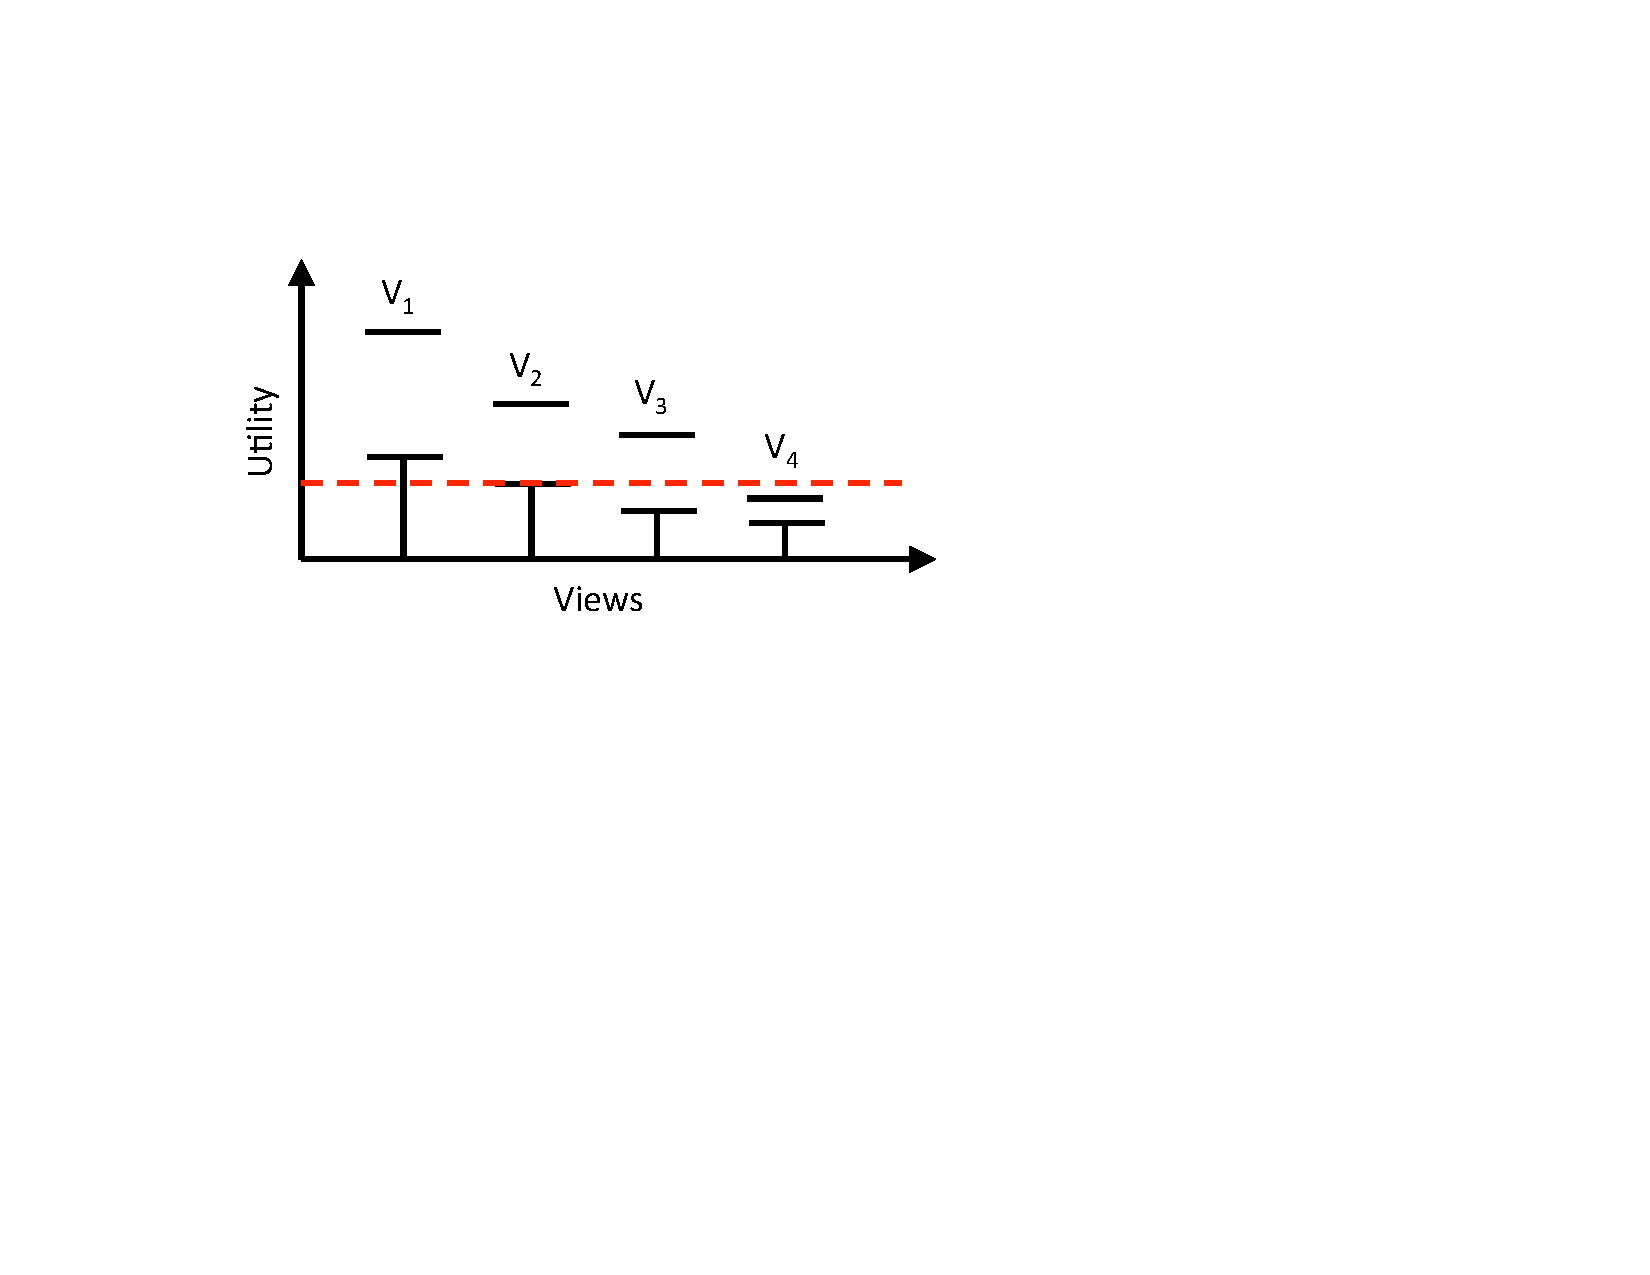
\includegraphics[trim=10mm 100mm 55mm 35mm, 
clip=true]{Images/confidence_pruning.pdf}}}}
\caption{Confidence Interval based Pruning}
\label{fig:conf_interval}
\vspace{-12pt}
\end{figure}


\stitle{Worst-Case Confidence Intervals.} 
Suppose we have $N$ values $y_1, \ldots, y_n$ in $[0, 1]$, and we are drawing
from them without replacement. 
Say we have drawn $m$ values so far, which are $Y_1, \ldots, Y_m$.
Then, we use the Hoeffding-Serfling inequality~\cite{serfling1974probability} 
to derive a running 
confidence interval such that the actual mean of the $N$
is always within the confidence interval with a probability of $\delta$:
\begin{theorem}
\label{thm:hs}
Let $\calY = y_1,$ $\ldots,$ $y_N$ be a set of $N$ 
values in $[0,1]$ with average value
$\frac1N \sum_{i=1}^N y_i = \mu$.
Let $Y_1,\ldots,Y_N$ be a 
sequence of random variables drawn from $\calY$ without
replacement.
Fix any $\delta > 0$. For $1 \le m \le N-1$, define
$$
\varepsilon_m = \sqrt{\frac{(1-\frac{m-1}N)(2\log \log (m) + \log(\pi^2/3\delta))}{2m}}.
$$
$$
\textrm{Then:} \ \   \Pr\left[ \exists m, 1 \le m \le N : 
  \left|\frac{\sum_{i=1}^m Y_i}{m} - \mu\right| > \varepsilon_m \right] 
\le \delta.
$$
\end{theorem}
In our setting, the current mean, $\sum Y_i / m$ is the 
the current estimate of the utility based on the samples seen thus far
for each view. 
Thus, to apply this pruning strategy, the only statistics
we need are the current estimate of the utilities.

Note that in this setting, we are assuming that since the
utility estimate at any stage of processing is in $[0, 1]$, 
the $Y_i$ values, i.e., the incremental contributions to the utility
that come from reading each record, are also between $[0, 1]$,
and are independent of the current value of the utility. 
This need not always hold. 
\agp{give example.}
Thus, the guarantees do not directly apply to our setting. 


\stitle{Normal Confidence Intervals.}
To apply this pruning strategy, we track 


\subsubsection{Normal Confidence Interval-Based Pruning}
\label{sec:confident_interval}
This pruning strategy is based on the application of sampling and confidence
intervals to utility estimates. First, as described above, we must specify
a set of statistics to track for each view and a rule that is used to
prune views based on the statistic.
For confidence interval based pruning, the statistics we track are the mean, 
variance, and confidence intervals of the view utility.
As \VizRecDB\ reads each record, it updates the data
distributions for all views and calculates the current utility of each view. 
Using past measures of utility, \VizRecDB\ also tracks the mean,
variance and confidence intervals for the utility of each view.
At the end of a phase, \VizRecDB\ uses the following rule for pruning low-utility
views (stated more formally below): {\it if the upperbound on the utility
of view $v_i$ is lesser than the least lowerbound on the utility of the
top-$k$ views, view $v_i$ is discarded.}

Let us dive deeper into this pruning rule.
Note that as we sequentially read records from a file, we are
approximating a sampling process (remember that the records are in random order).
For instance, suppose that we have read 10K records from a 1M record file.
In this case, the records 1 -- 10K constitute a 1\% sample of the entire file.
When we read the next say 10 records, the records 1 -- 10,010 constitute an
incrementally larger sample of the underlying file.
Thus, as we read more data from the file, we obtaining a large
number of samples from the underlying data (notice however, that these samples
are not independent).

Since we are generating a large number of samples from a population, we can
invoke a well-studied concept in statistics called the ``sampling distribution.'' 
A sampling distribution for a statistic $S$ is the distribution of
$S$ generated by taking a large number of samples of a fixed size and computing
the statistic $S$ on each sample.
In our case, the population we draw from is the set of all records in the file
and our samples are the increasingly larger sets of records that we are reading in.
The statistic $S$ that we are computing is the view utility (we
compute a utility value for each view).
Now, the sampling distribution of the {\it mean} has been well studied and it
has been proven that the mean of the sampling distribution is equal to the mean of the
population and the standard error of the sampling distribution is equal to the
standard error of the population divided by the square root of the sample size. 
These two formulas are shown in Equations \ref{eq:mean} and \ref{eq:variance}.
Similarly, if we know the mean and standard error of the sampling distribution,
we can compute a confidence interval around the population mean. This is shown
in Equation \ref{eq:confidence_interval} where $z$ is the factor that depends on the
confidence threshold we are aiming for and $N$ is the number of items
in each sample.

\begin{eqnarray}
\label{eqnarray:mean_and_variance}
\mu_M = \mu \label{eq:mean}\\
\sigma_{M} = \frac{\sigma}{\sqrt{N}} \label{eq:variance}\\
CI = \mu_M \pm z \ast \frac{\sigma_M}{\sqrt{N}}\label{eq:confidence_interval}
\end{eqnarray}

If we were modeling the mean of our samples instead of the utility, we could use
the above result directly.
However, we find that with a few minor modifications, we can use the confidence
interval bounds shown above.
The first modification we make has to do with how we define utility.
Remember from Section \ref{sec:problem_definition} that the utility of a view is
defined as the distance between two distributions: the distribution of aggregate values for the
target view and the distribution of aggregate values for the comparison view.
These distributions are in turn tied to the number of distinct groups present in
each dimension attribute.
For our purposes, it means that if a dimension attribute has $n$ distinct
groups, then a sample with $x$ rows gives us approximately $\frac{x}{n}$ values
for each group (assuming uniform distribution).
Said another way, a sample with $x$ rows for the purpose of computing utility is
really only a sample of $\frac{x}{n}$ rows.
So the first modification we make to Equation \ref{eq:confidence_interval} is to
replace $N$ by $\frac{N}{G_{max}}$ where $G_{max}$ is the maximum number of
distinct groups present in any dimension attribute.
Second, we observe that the sampling distribution applies to the case where
samples are of the same size and are independently generated.
This is not true in our algorithm; therefore, to compensate, make two
conservative modifications: we set $N$ to the number of rows that
have been read in the previous phase (remember that pruning happens at the end
of every phase) and we set the $z$ parameter to a value $\geq$ 1.96 (the normal
95\% confidence interval value). These modifications ensure (as we will show
empirically in Section \ref{sec:experiments}) that the confidence intervals
always contain the mean and continually shrink as we read in more data.



% Now that we have a way of finding confidence intervals, we elaborate on how we
% use them to perfom pruning.
% Suppose at the end of phase $p$ the confidence intervals for the views in
% running have values shown in Figure \ref{fig:conf_interval} and we want to
% identify the two views with the highest utility.
% Consider view $V_3$, we see that its confidence interval overlaps with the
% confidence intervals of the current top views $V_1$ and $V_2$, making it likely
% that $V_3$ will be in the final top views. On the other hand, the confidence
% interval for $V_4$ lies entirely below the lowest bound of the top two
% intervals.
% Since we can claim with high probability (depending on the confidence threshold)
% that the utility of $V_4$ lies within its confidence interval, it follows that
% with high probability, $V_4$ will not appear in the top-$2$ views.
% This is essentially our pruning rule. 
% We state the algorithm fomally in
% Algorithm \ref{algo:ci_based_pruning}.

\begin{algorithm}
\caption{Confidence Interval Based Pruning}
\label{algo:ci_based_pruning}
\begin{algorithmic}[1]
\State viewsInRunning.sortByUpperbound()
\State topViews $\gets$ viewsInRunning.getTopK()
\State lowestLowerbound $\gets$ min(lowerbound(topViews))
\For {view $\not \in$ topViews}
\If {view.upperbound < lowestLowerbound}
\State viewsInRunning.remove(view)
\EndIf
\EndFor
\end{algorithmic}
\end{algorithm}

\subsubsection{Multi-Armed Bandit Pruning}
\label{sec:multi_armed_bandit}
The second class of pruning techniques we explore are based on a
well-known learning problem called the ``Multi-Armed Bandit'' (MAB).
The MAB setting is as follows: a gambler is faced with several slot
machines (``one armed bandits'') that each have an underlying reward
distribution. 
The gambler has some number of turns at the slot machines and at
each turn, the gambler must decide which machine to play in order to maximize
the total reward.
Recently, variants of MAB have been proposed which instead of maximizing total
reward, focus on finding the bandits with the highest
mean reward (\cite{}).
This is very similar to our setting: each possible view can be thought of as a
one-armed bandit and our goal is find the views with the highest reward (i.e.
utility).
As with the confidence interval based pruning, we consider the sequential
reading of our file to be similar to random sampling with increasing sample
size.
In MAB, each pull of an arm (i.e. slot machine) corresponds to a drawing from
the underlying probability distribution of that slot machine.
In our case, each new value for a particular pair of attributes (1 dimension and
1 measure) corresponds to a drawing from the underlying utility distribution
of that view.
There are two approximations we make here: (1) although the utility of a
view is ultimately a single value, we can approximate it as probability
distribution that is normally distributed around the true utility and has a
small standard deviation, and (2) when we read the $i$-th record, instead of
pulling from the probability distribution discussed above, we are pulling from a
sampling distribution of the utility with sample size $i$.

As a result, the MAB setting doesn't translate directly to our case. 
However, as we show in our experimental evaluation, the approximation works well
in real settings.
Algorithm \ref{algo:mab_based_pruning} shows the pruning technique used in the
MAB setting.
This
algorithm is an adaptation of Successive Accepts and Rejects
algorithm from \cite{BubeckWV13} for finding the top-$k$ arms with the highest
mean reward.
As before, the processing of the whole file is divided into phases, with the
number of phases set to $k$-1 for this heuristic.
As opposed to the confidence interval heuristic, we only track a single
statistic for MAB, namely the utility mean.
At the end of every phase, we adopt the following pruning technique: all views
in running are ranked in order of their utility means. 
We then compute two special differences between the utility means: $\Delta_1$
is the difference between the highest mean and the $k+1$st highest mean, and
$\Delta_n$ is the difference between the lowest mean and the $k$th highest mean.
If $\Delta_1$ is greater than $\Delta_n$, the view with the highest mean is
{\it accepted} as being part of the the top-$k$ (and it no longer participates
in pruning computations).
On the otherhand, if $\Delta_n$ is higher, the view with the lowest mean is discarded
from the set of views in the running.
Note again that if the number of views in the running is equal to $k$, it is
possible to stop early and provide the user an approximate set of views.

\begin{algorithm}
\caption{MAB Based Pruning}
\label{algo:mab_based_pruning}
\begin{algorithmic}[1]
\State viewsInRunning.sortByUtilityMean()
\State \{$\bar{u}_{i}$\} $\gets$ sorted utility means
\State $\Delta_1$ $\gets$ $\bar{u}_{1}$ - $\bar{u}_{k+1}$
\State $\Delta_n$ $\gets$ $\bar{u}_{k}$ - $\bar{u}_{n}$
\If {$\Delta_1$ < $\Delta_n$}
\State viewsInRunning.acceptTop()
\Else
\State viewsInRunning.discardBottom()
\EndIf
\end{algorithmic}
\end{algorithm}

\cite{BubeckWV13} provides bounds on the optimality of this heuristic for the
MAB setting.
Since our problem setup isn't exactly the same, the optimality bounds don't
transfer directly.
However, as we show in the experimental section, the MAB heuristic performs well
on real datasets.

\subsubsection{Incorportating Custom Engine into a DBMS}
\label{sec:incorporating}
\mpv{Do we want this section?}
In an ideal solution, we would incorporate the algorithms used in our custom
engine into a DBMS. 
The advantages of integrating into a DBMS are clear: we could take advantage of
the superior data storage and retrieval techniques in databases, and we would
avoid building a one-off, super-specialized system.
However, as the current database API stands, there is no way to share table
scans between operations, keep track of custom statistics or intercept the scan
mid-way to perform pruning.
If we are two implement a \VizRecDB-style operator in a traditional database
system, we would have to support the following operations:
\squishlist
\item Ability to store custom state during aggregation operations (e.g.
distributions corresponding to each view)
\item Ability to compute custom statistics during a table scan (in our case
utilities, their cummulative means and variances)
\item Ability to compute multiple aggregates and group-bys at the same time
(similar to the GROUPING SETS functionality)
\item Ability to intercept the scan periodically (think of a call back or a
sleep functionality) in order to update the custom state
\squishend

These operators can be embedded in the query executor or as part of a UDF.
We lay down these requirements because we expect that not just \VizRecDB\ but
other kinds of similar workloads would also benefit from such an API.
This implementation is out of scope for the current work, but we plan to explore
it in future work.
